\documentclass[a4paper]{article}
\usepackage[UTF8]{ctex}
\usepackage{graphicx}

\title{双链列表的模型与实现}
\author{李沁霞 \\ 统计学 3210300363}
\date{\today}

\begin{document}

\maketitle

\section{项目要求}
实现 DoubleLinkedList<DT> 的基本操作,使用find, erase, delete等函数实现双链表的基本功能,测试代码完备性,并检查代码的内存泄漏。

\section{设计思路}
\begin{enumerate}
    \item 首先,编写find外部函数,用于找到该除的函数位置。
    \item 然后,构造PrintList void函数,用于输出迭代器。
    \item 最后,编写main函数进行程序测试。
\end{enumerate}

\section{实现代码解释}
\begin{enumerate}
    \item find外部函数
    \begin{center}
        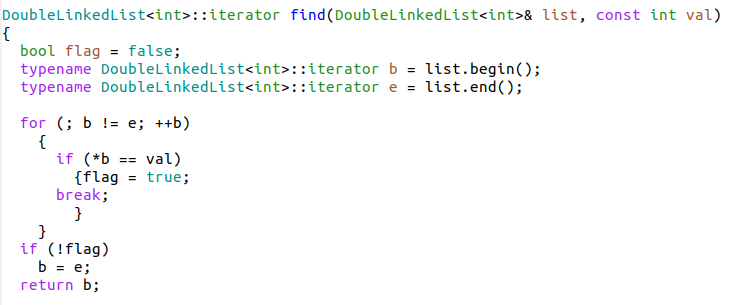
\includegraphics[width=13cm,scale=0.55]{find}
    \end{center}
    \item PrintList void函数
    \begin{center}
        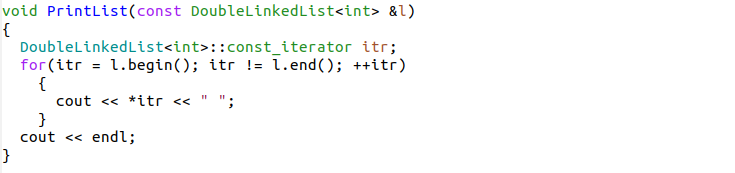
\includegraphics[width=13cm,scale=0.6]{PrintList}
    \end{center}
    \item main函数
    \begin{center}
        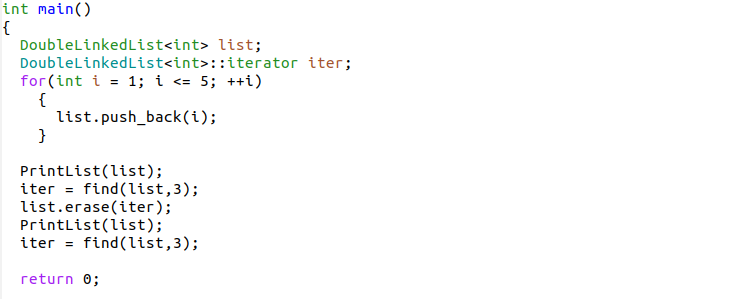
\includegraphics[width=13.5cm, scale=0.7]{main}
    \end{center}
\end{enumerate}

\section{测试结果及内存泄漏检查}
测试结果:
\begin{center}
    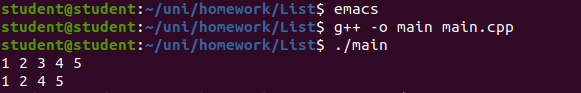
\includegraphics[width=12cm, scale=0.7]{result}
\end{center}
使用g++ -o main main.cpp测试代码的完备性,然后实现测试结果。显然,输入函数与输出不同。因为,在main代码中有实现erase列表的第3个位置。于是,输出函数剩下4个。\\

内存泄漏检查:
\begin{center}
    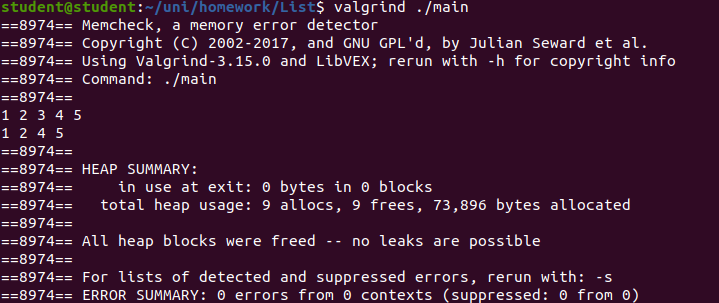
\includegraphics[width=13cm, scale=0.7]{memory}
\end{center}
使用valgrind函数检查内存泄漏。显然,以上代码不存在内存泄漏。

\end{document}
